% J. R. Capablanca - D. Janowski, St. Petersburg, 1914, with Capablanca's notes.
% Build with: python3 ../../tools/chessbook.py game-11-capablanca-janowski.tex
\documentclass[10pt,twoside]{article}
\usepackage[paperwidth=487.56bp,paperheight=691.65bp,top=72pt,bottom=44pt,inner=50pt,outer=48pt,
            headheight=13pt,headsep=20pt,footskip=0pt]{geometry}
\usepackage[T1]{fontenc}
\usepackage[lining]{ebgaramond}
\usepackage{graphicx}
\usepackage{microtype}
\usepackage{tikz}
\usepackage{fancyhdr}
\usepackage[hidelinks,pdftitle={Capablanca - Janowski, St. Petersburg, 1914},
            pdfauthor={J. R. Capablanca}]{hyperref}

\newcommand{\textsizebook}{\fontsize{10.5}{12.6}\selectfont}
\AtBeginDocument{\textsizebook}
\setlength{\columnsep}{11pt}
\setlength{\parindent}{9pt}
\setlength{\parskip}{0pt}
\setlength{\emergencystretch}{1.5em}
\raggedbottom

\newlength{\boardwidth}
\setlength{\boardwidth}{160pt}

% A main line move, as a bold heading above its note
\newcommand{\Move}[1]{\par\addvspace{8pt}\noindent\phantomsection{\bfseries #1}\par\nopagebreak}
% A diagram in the text
\newcommand{\ChessDiagram}[1]{\par\addvspace{7pt}{\centering #1\par}\addvspace{5pt}}

\pagestyle{fancy}
\fancyhf{}
\renewcommand{\headrulewidth}{0pt}
\fancyhead[LE,RO]{\thepage}
\fancyhead[CE]{Ruy Lopez}
\fancyhead[CO]{Capablanca -- Janowski}





\newcommand{\figK}{\raisebox{-0.14em}{
\includegraphics[height=1em]{diagrams/figK}}}
\newcommand{\figQ}{\raisebox{-0.14em}{
\includegraphics[height=1em]{diagrams/figQ}}}
\newcommand{\figR}{\raisebox{-0.14em}{
\includegraphics[height=1em]{diagrams/figR}}}
\newcommand{\figB}{\raisebox{-0.14em}{
\includegraphics[height=1em]{diagrams/figB}}}
\newcommand{\figN}{\raisebox{-0.14em}{
\includegraphics[height=1em]{diagrams/figN}}}
\begin{document}

\twocolumn[{%
\thispagestyle{empty}
\begin{tikzpicture}[remember picture,overlay]
  \node[circle,draw=black,line width=1.6pt,fill=black!20,minimum size=112pt] (seal)
       at ([xshift=75pt,yshift=-75pt]current page.north west) {};
  \draw[line width=0.9pt] ([shift={(-48pt,-30pt)}]seal.center) -- ([shift={(44pt,34pt)}]seal.center);
  \node[rotate=37] at ([shift={(-11pt,14pt)}]seal.center) {\fontsize{25}{25}\selectfont\bfseries Game};
  \node[rotate=37] at ([shift={(10pt,-16pt)}]seal.center) {\fontsize{38}{38}\selectfont\bfseries 11};
  \node[anchor=north east] at ([xshift=-14pt,yshift=-24pt]current page.north east)
       {\href{https://lichess.org/analysis/pgn/e4_e5_Nf3_Nc6_Bb5_a6_Bxc6_dxc6}{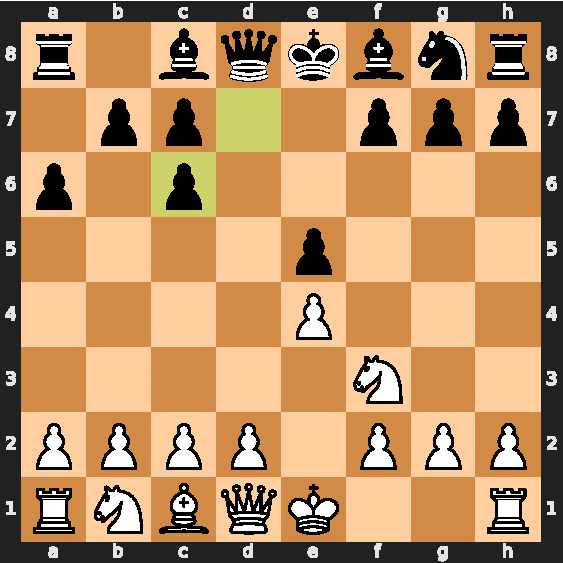
\includegraphics[width=108pt]{diagrams/board-8e9ff290c4c2}}};
\end{tikzpicture}

\vspace*{38pt}
\begin{center}
  \begin{minipage}{235pt}\centering
    {\fontsize{22}{25}\selectfont\bfseries Ruy Lopez\par}
    \vspace{4pt}\rule{\linewidth}{1pt}\\[-9.5pt]\rule{\linewidth}{0.4pt}
  \end{minipage}

  \vspace{14pt}
  {\fontsize{19}{22}\selectfont\bfseries Capablanca -- Janowski\par}
  \vspace{10pt}
  {\fontsize{15}{18}\selectfont\bfseries St. Petersburg, 1914\par}
  \vspace{8pt}
  {\fontsize{11}{13}\selectfont White: J. R. Capablanca \quad Black: D. Janowski\par}
  \vspace{10pt}
  {\centering\fontsize{8.5}{10}\selectfont\itshape
   Notes by J. R. Capablanca, from \textup{Chess Fundamentals} (1921), which is in the public domain.\\
   Descriptive notation has been converted to algebraic. Page references are to the book.\\
   Click any move or diagram to open it on Lichess.\par}
\end{center}
\vspace{10pt}
}]
\textsizebook

\Move{\href{https://lichess.org/analysis/pgn/e4}{1.e4} \href{https://lichess.org/analysis/pgn/e4_e5}{e5} \href{https://lichess.org/analysis/pgn/e4_e5_Nf3}{2.\figN f3} \href{https://lichess.org/analysis/pgn/e4_e5_Nf3_Nc6}{\figN c6} \href{https://lichess.org/analysis/pgn/e4_e5_Nf3_Nc6_Bb5}{3.\figB b5} \href{https://lichess.org/analysis/pgn/e4_e5_Nf3_Nc6_Bb5_a6}{a6} \href{https://lichess.org/analysis/pgn/e4_e5_Nf3_Nc6_Bb5_a6_Bxc6}{4.\figB xc6} \href{https://lichess.org/analysis/pgn/e4_e5_Nf3_Nc6_Bb5_a6_Bxc6_dxc6}{dxc6} \href{https://lichess.org/analysis/pgn/e4_e5_Nf3_Nc6_Bb5_a6_Bxc6_dxc6_Nc3}{5.\figN c3}}

I played this move after having discussed it with Alechin on several occasions. Alechin considered it, at the time, superior to \href{https://lichess.org/analysis/pgn/e4_e5_Nf3_Nc6_Bb5_a6_Bxc6_dxc6_d4}{5.d4}, which is generally played. He played it himself later on in the Tournament, in one of his games against Dr. E. Lasker, and obtained the superior game, which he only lost through a blunder.

\Move{\href{https://lichess.org/analysis/pgn/e4_e5_Nf3_Nc6_Bb5_a6_Bxc6_dxc6_Nc3_Bc5}{5...\figB c5}}

\href{https://lichess.org/analysis/pgn/e4_e5_Nf3_Nc6_Bb5_a6_Bxc6_dxc6_Nc3_f6}{5...f6} is probably the best move in this position. I do not like the text move.

\Move{\href{https://lichess.org/analysis/pgn/e4_e5_Nf3_Nc6_Bb5_a6_Bxc6_dxc6_Nc3_Bc5_d3}{6.d3} \href{https://lichess.org/analysis/pgn/e4_e5_Nf3_Nc6_Bb5_a6_Bxc6_dxc6_Nc3_Bc5_d3_Bg4}{\figB g4} \href{https://lichess.org/analysis/pgn/e4_e5_Nf3_Nc6_Bb5_a6_Bxc6_dxc6_Nc3_Bc5_d3_Bg4_Be3}{7.\figB e3} \href{https://lichess.org/analysis/pgn/e4_e5_Nf3_Nc6_Bb5_a6_Bxc6_dxc6_Nc3_Bc5_d3_Bg4_Be3_Bxe3}{\figB xe3}}

This opens the f-file for White, and also reinforces his centre, but Black naturally did not want to make a second move with this Bishop.

\Move{\href{https://lichess.org/analysis/pgn/e4_e5_Nf3_Nc6_Bb5_a6_Bxc6_dxc6_Nc3_Bc5_d3_Bg4_Be3_Bxe3_fxe3}{8.fxe3} \href{https://lichess.org/analysis/pgn/e4_e5_Nf3_Nc6_Bb5_a6_Bxc6_dxc6_Nc3_Bc5_d3_Bg4_Be3_Bxe3_fxe3_Qe7}{\figQ e7} \href{https://lichess.org/analysis/pgn/e4_e5_Nf3_Nc6_Bb5_a6_Bxc6_dxc6_Nc3_Bc5_d3_Bg4_Be3_Bxe3_fxe3_Qe7_O-O}{9.0--0} \href{https://lichess.org/analysis/pgn/e4_e5_Nf3_Nc6_Bb5_a6_Bxc6_dxc6_Nc3_Bc5_d3_Bg4_Be3_Bxe3_fxe3_Qe7_O-O_O-O-O}{0--0--0}}

Bold play, typical of Janowski.

\Move{\href{https://lichess.org/analysis/pgn/e4_e5_Nf3_Nc6_Bb5_a6_Bxc6_dxc6_Nc3_Bc5_d3_Bg4_Be3_Bxe3_fxe3_Qe7_O-O_O-O-O_Qe1}{10.\figQ e1} \href{https://lichess.org/analysis/pgn/e4_e5_Nf3_Nc6_Bb5_a6_Bxc6_dxc6_Nc3_Bc5_d3_Bg4_Be3_Bxe3_fxe3_Qe7_O-O_O-O-O_Qe1_Nh6}{\figN h6}}

\ChessDiagram{\href{https://lichess.org/analysis/pgn/e4_e5_Nf3_Nc6_Bb5_a6_Bxc6_dxc6_Nc3_Bc5_d3_Bg4_Be3_Bxe3_fxe3_Qe7_O-O_O-O-O_Qe1_Nh6}{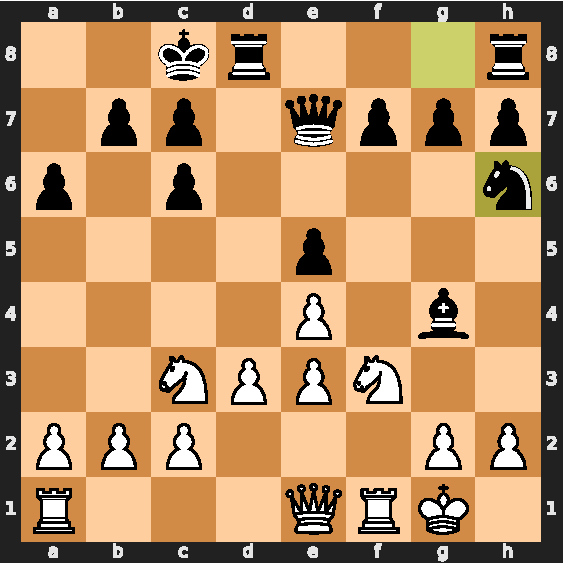
\includegraphics[width=\boardwidth]{diagrams/board-02d9729686e1}}}

The problem for White now is to advance his b-pawn to b5 as fast as he can. If he plays \href{https://lichess.org/analysis/pgn/e4_e5_Nf3_Nc6_Bb5_a6_Bxc6_dxc6_Nc3_Bc5_d3_Bg4_Be3_Bxe3_fxe3_Qe7_O-O_O-O-O_Qe1_Nh6_b4}{11.b4} at once, Black simply takes it. If he plays first a3 and then b4, he will still have to protect his b-pawn before he can go on and play a4 and b5. As a matter of fact White played a rather unusual move, but one which, under the circumstances, was the best, since after it he could at once play b4 and then a4 and b5.

\Move{\href{https://lichess.org/analysis/pgn/e4_e5_Nf3_Nc6_Bb5_a6_Bxc6_dxc6_Nc3_Bc5_d3_Bg4_Be3_Bxe3_fxe3_Qe7_O-O_O-O-O_Qe1_Nh6_Rb1}{11.\figR b1!} \href{https://lichess.org/analysis/pgn/e4_e5_Nf3_Nc6_Bb5_a6_Bxc6_dxc6_Nc3_Bc5_d3_Bg4_Be3_Bxe3_fxe3_Qe7_O-O_O-O-O_Qe1_Nh6_Rb1_f6}{f6} \href{https://lichess.org/analysis/pgn/e4_e5_Nf3_Nc6_Bb5_a6_Bxc6_dxc6_Nc3_Bc5_d3_Bg4_Be3_Bxe3_fxe3_Qe7_O-O_O-O-O_Qe1_Nh6_Rb1_f6_b4}{12.b4} \href{https://lichess.org/analysis/pgn/e4_e5_Nf3_Nc6_Bb5_a6_Bxc6_dxc6_Nc3_Bc5_d3_Bg4_Be3_Bxe3_fxe3_Qe7_O-O_O-O-O_Qe1_Nh6_Rb1_f6_b4_Nf7}{\figN f7} \href{https://lichess.org/analysis/pgn/e4_e5_Nf3_Nc6_Bb5_a6_Bxc6_dxc6_Nc3_Bc5_d3_Bg4_Be3_Bxe3_fxe3_Qe7_O-O_O-O-O_Qe1_Nh6_Rb1_f6_b4_Nf7_a4}{13.a4} \href{https://lichess.org/analysis/pgn/e4_e5_Nf3_Nc6_Bb5_a6_Bxc6_dxc6_Nc3_Bc5_d3_Bg4_Be3_Bxe3_fxe3_Qe7_O-O_O-O-O_Qe1_Nh6_Rb1_f6_b4_Nf7_a4_Bxf3}{\figB xf3}}

He simplifies, hoping to lighten White's attack, which will have to be conducted practically with only the heavy pieces on the board. He may have also done it in order to play \figN g5 and e6.

\Move{\href{https://lichess.org/analysis/pgn/e4_e5_Nf3_Nc6_Bb5_a6_Bxc6_dxc6_Nc3_Bc5_d3_Bg4_Be3_Bxe3_fxe3_Qe7_O-O_O-O-O_Qe1_Nh6_Rb1_f6_b4_Nf7_a4_Bxf3_Rxf3}{14.\figR xf3}}

Taking with the Pawn would have opened a possibility for a counter attack.

\Move{\href{https://lichess.org/analysis/pgn/e4_e5_Nf3_Nc6_Bb5_a6_Bxc6_dxc6_Nc3_Bc5_d3_Bg4_Be3_Bxe3_fxe3_Qe7_O-O_O-O-O_Qe1_Nh6_Rb1_f6_b4_Nf7_a4_Bxf3_Rxf3_b6}{14...b6}}

He is forced to this in order to avoid the breaking up of his Queen's side Pawns. The only alternative would have been \href{https://lichess.org/analysis/pgn/e4_e5_Nf3_Nc6_Bb5_a6_Bxc6_dxc6_Nc3_Bc5_d3_Bg4_Be3_Bxe3_fxe3_Qe7_O-O_O-O-O_Qe1_Nh6_Rb1_f6_b4_Nf7_a4_Bxf3_Rxf3_b5}{14...b5}; which on the face of it looks bad.

\Move{\href{https://lichess.org/analysis/pgn/e4_e5_Nf3_Nc6_Bb5_a6_Bxc6_dxc6_Nc3_Bc5_d3_Bg4_Be3_Bxe3_fxe3_Qe7_O-O_O-O-O_Qe1_Nh6_Rb1_f6_b4_Nf7_a4_Bxf3_Rxf3_b6_b5}{15.b5} \href{https://lichess.org/analysis/pgn/e4_e5_Nf3_Nc6_Bb5_a6_Bxc6_dxc6_Nc3_Bc5_d3_Bg4_Be3_Bxe3_fxe3_Qe7_O-O_O-O-O_Qe1_Nh6_Rb1_f6_b4_Nf7_a4_Bxf3_Rxf3_b6_b5_cxb5}{cxb5} \href{https://lichess.org/analysis/pgn/e4_e5_Nf3_Nc6_Bb5_a6_Bxc6_dxc6_Nc3_Bc5_d3_Bg4_Be3_Bxe3_fxe3_Qe7_O-O_O-O-O_Qe1_Nh6_Rb1_f6_b4_Nf7_a4_Bxf3_Rxf3_b6_b5_cxb5_axb5}{16.axb5} \href{https://lichess.org/analysis/pgn/e4_e5_Nf3_Nc6_Bb5_a6_Bxc6_dxc6_Nc3_Bc5_d3_Bg4_Be3_Bxe3_fxe3_Qe7_O-O_O-O-O_Qe1_Nh6_Rb1_f6_b4_Nf7_a4_Bxf3_Rxf3_b6_b5_cxb5_axb5_a5}{a5} \href{https://lichess.org/analysis/pgn/e4_e5_Nf3_Nc6_Bb5_a6_Bxc6_dxc6_Nc3_Bc5_d3_Bg4_Be3_Bxe3_fxe3_Qe7_O-O_O-O-O_Qe1_Nh6_Rb1_f6_b4_Nf7_a4_Bxf3_Rxf3_b6_b5_cxb5_axb5_a5_Nd5}{17.\figN d5} \href{https://lichess.org/analysis/pgn/e4_e5_Nf3_Nc6_Bb5_a6_Bxc6_dxc6_Nc3_Bc5_d3_Bg4_Be3_Bxe3_fxe3_Qe7_O-O_O-O-O_Qe1_Nh6_Rb1_f6_b4_Nf7_a4_Bxf3_Rxf3_b6_b5_cxb5_axb5_a5_Nd5_Qc5}{\figQ c5} \href{https://lichess.org/analysis/pgn/e4_e5_Nf3_Nc6_Bb5_a6_Bxc6_dxc6_Nc3_Bc5_d3_Bg4_Be3_Bxe3_fxe3_Qe7_O-O_O-O-O_Qe1_Nh6_Rb1_f6_b4_Nf7_a4_Bxf3_Rxf3_b6_b5_cxb5_axb5_a5_Nd5_Qc5_c4}{18.c4}}

\ChessDiagram{\href{https://lichess.org/analysis/pgn/e4_e5_Nf3_Nc6_Bb5_a6_Bxc6_dxc6_Nc3_Bc5_d3_Bg4_Be3_Bxe3_fxe3_Qe7_O-O_O-O-O_Qe1_Nh6_Rb1_f6_b4_Nf7_a4_Bxf3_Rxf3_b6_b5_cxb5_axb5_a5_Nd5_Qc5_c4}{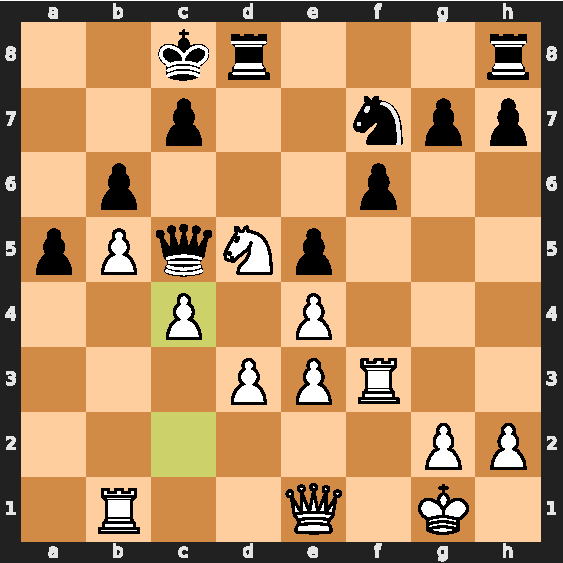
\includegraphics[width=\boardwidth]{diagrams/board-af66d70fdd83}}}

The White Knight is now a tower of strength. Behind it White will be able to prepare an attack, which will begin with d4, to drive away the Black Queen and thus leave himself free to play c5. There is only one thing to take care of and that is to prevent Black from sacrificing the Rook for the Knight and a Pawn.

\Move{\href{https://lichess.org/analysis/pgn/e4_e5_Nf3_Nc6_Bb5_a6_Bxc6_dxc6_Nc3_Bc5_d3_Bg4_Be3_Bxe3_fxe3_Qe7_O-O_O-O-O_Qe1_Nh6_Rb1_f6_b4_Nf7_a4_Bxf3_Rxf3_b6_b5_cxb5_axb5_a5_Nd5_Qc5_c4_Ng5}{18...\figN g5} \href{https://lichess.org/analysis/pgn/e4_e5_Nf3_Nc6_Bb5_a6_Bxc6_dxc6_Nc3_Bc5_d3_Bg4_Be3_Bxe3_fxe3_Qe7_O-O_O-O-O_Qe1_Nh6_Rb1_f6_b4_Nf7_a4_Bxf3_Rxf3_b6_b5_cxb5_axb5_a5_Nd5_Qc5_c4_Ng5_Rf2}{19.\figR f2} \href{https://lichess.org/analysis/pgn/e4_e5_Nf3_Nc6_Bb5_a6_Bxc6_dxc6_Nc3_Bc5_d3_Bg4_Be3_Bxe3_fxe3_Qe7_O-O_O-O-O_Qe1_Nh6_Rb1_f6_b4_Nf7_a4_Bxf3_Rxf3_b6_b5_cxb5_axb5_a5_Nd5_Qc5_c4_Ng5_Rf2_Ne6}{\figN e6} \href{https://lichess.org/analysis/pgn/e4_e5_Nf3_Nc6_Bb5_a6_Bxc6_dxc6_Nc3_Bc5_d3_Bg4_Be3_Bxe3_fxe3_Qe7_O-O_O-O-O_Qe1_Nh6_Rb1_f6_b4_Nf7_a4_Bxf3_Rxf3_b6_b5_cxb5_axb5_a5_Nd5_Qc5_c4_Ng5_Rf2_Ne6_Qc3}{20.\figQ c3} \href{https://lichess.org/analysis/pgn/e4_e5_Nf3_Nc6_Bb5_a6_Bxc6_dxc6_Nc3_Bc5_d3_Bg4_Be3_Bxe3_fxe3_Qe7_O-O_O-O-O_Qe1_Nh6_Rb1_f6_b4_Nf7_a4_Bxf3_Rxf3_b6_b5_cxb5_axb5_a5_Nd5_Qc5_c4_Ng5_Rf2_Ne6_Qc3_Rd7}{\figR d7}}

Had White on his 19th move played \href{https://lichess.org/analysis/pgn/e4_e5_Nf3_Nc6_Bb5_a6_Bxc6_dxc6_Nc3_Bc5_d3_Bg4_Be3_Bxe3_fxe3_Qe7_O-O_O-O-O_Qe1_Nh6_Rb1_f6_b4_Nf7_a4_Bxf3_Rxf3_b6_b5_cxb5_axb5_a5_Nd5_Qc5_c4_Ng5_Rf1}{19.\figR f1} instead of \href{https://lichess.org/analysis/pgn/e4_e5_Nf3_Nc6_Bb5_a6_Bxc6_dxc6_Nc3_Bc5_d3_Bg4_Be3_Bxe3_fxe3_Qe7_O-O_O-O-O_Qe1_Nh6_Rb1_f6_b4_Nf7_a4_Bxf3_Rxf3_b6_b5_cxb5_axb5_a5_Nd5_Qc5_c4_Ng5_Rf2}{19.\figR f2}, Black could have played now instead of the text move, \figR xd5; exd5, \figQ xe3+; followed by \figN f4 with a winning game.

\Move{\href{https://lichess.org/analysis/pgn/e4_e5_Nf3_Nc6_Bb5_a6_Bxc6_dxc6_Nc3_Bc5_d3_Bg4_Be3_Bxe3_fxe3_Qe7_O-O_O-O-O_Qe1_Nh6_Rb1_f6_b4_Nf7_a4_Bxf3_Rxf3_b6_b5_cxb5_axb5_a5_Nd5_Qc5_c4_Ng5_Rf2_Ne6_Qc3_Rd7_Rd1}{21.\figR d1} \href{https://lichess.org/analysis/pgn/e4_e5_Nf3_Nc6_Bb5_a6_Bxc6_dxc6_Nc3_Bc5_d3_Bg4_Be3_Bxe3_fxe3_Qe7_O-O_O-O-O_Qe1_Nh6_Rb1_f6_b4_Nf7_a4_Bxf3_Rxf3_b6_b5_cxb5_axb5_a5_Nd5_Qc5_c4_Ng5_Rf2_Ne6_Qc3_Rd7_Rd1_Kb7}{\figK b7}}

It would have been better for Black to play \href{https://lichess.org/analysis/pgn/e4_e5_Nf3_Nc6_Bb5_a6_Bxc6_dxc6_Nc3_Bc5_d3_Bg4_Be3_Bxe3_fxe3_Qe7_O-O_O-O-O_Qe1_Nh6_Rb1_f6_b4_Nf7_a4_Bxf3_Rxf3_b6_b5_cxb5_axb5_a5_Nd5_Qc5_c4_Ng5_Rf2_Ne6_Qc3_Rd7_Rd1_Kd8}{21...\figK d8}. The text move loses very rapidly.

\Move{\href{https://lichess.org/analysis/pgn/e4_e5_Nf3_Nc6_Bb5_a6_Bxc6_dxc6_Nc3_Bc5_d3_Bg4_Be3_Bxe3_fxe3_Qe7_O-O_O-O-O_Qe1_Nh6_Rb1_f6_b4_Nf7_a4_Bxf3_Rxf3_b6_b5_cxb5_axb5_a5_Nd5_Qc5_c4_Ng5_Rf2_Ne6_Qc3_Rd7_Rd1_Kb7_d4}{22.d4} \href{https://lichess.org/analysis/pgn/e4_e5_Nf3_Nc6_Bb5_a6_Bxc6_dxc6_Nc3_Bc5_d3_Bg4_Be3_Bxe3_fxe3_Qe7_O-O_O-O-O_Qe1_Nh6_Rb1_f6_b4_Nf7_a4_Bxf3_Rxf3_b6_b5_cxb5_axb5_a5_Nd5_Qc5_c4_Ng5_Rf2_Ne6_Qc3_Rd7_Rd1_Kb7_d4_Qd6}{\figQ d6} \href{https://lichess.org/analysis/pgn/e4_e5_Nf3_Nc6_Bb5_a6_Bxc6_dxc6_Nc3_Bc5_d3_Bg4_Be3_Bxe3_fxe3_Qe7_O-O_O-O-O_Qe1_Nh6_Rb1_f6_b4_Nf7_a4_Bxf3_Rxf3_b6_b5_cxb5_axb5_a5_Nd5_Qc5_c4_Ng5_Rf2_Ne6_Qc3_Rd7_Rd1_Kb7_d4_Qd6_Rc2}{23.\figR c2} \href{https://lichess.org/analysis/pgn/e4_e5_Nf3_Nc6_Bb5_a6_Bxc6_dxc6_Nc3_Bc5_d3_Bg4_Be3_Bxe3_fxe3_Qe7_O-O_O-O-O_Qe1_Nh6_Rb1_f6_b4_Nf7_a4_Bxf3_Rxf3_b6_b5_cxb5_axb5_a5_Nd5_Qc5_c4_Ng5_Rf2_Ne6_Qc3_Rd7_Rd1_Kb7_d4_Qd6_Rc2_exd4}{exd4} \href{https://lichess.org/analysis/pgn/e4_e5_Nf3_Nc6_Bb5_a6_Bxc6_dxc6_Nc3_Bc5_d3_Bg4_Be3_Bxe3_fxe3_Qe7_O-O_O-O-O_Qe1_Nh6_Rb1_f6_b4_Nf7_a4_Bxf3_Rxf3_b6_b5_cxb5_axb5_a5_Nd5_Qc5_c4_Ng5_Rf2_Ne6_Qc3_Rd7_Rd1_Kb7_d4_Qd6_Rc2_exd4_exd4}{24.exd4} \href{https://lichess.org/analysis/pgn/e4_e5_Nf3_Nc6_Bb5_a6_Bxc6_dxc6_Nc3_Bc5_d3_Bg4_Be3_Bxe3_fxe3_Qe7_O-O_O-O-O_Qe1_Nh6_Rb1_f6_b4_Nf7_a4_Bxf3_Rxf3_b6_b5_cxb5_axb5_a5_Nd5_Qc5_c4_Ng5_Rf2_Ne6_Qc3_Rd7_Rd1_Kb7_d4_Qd6_Rc2_exd4_exd4_Nf4}{\figN f4} \href{https://lichess.org/analysis/pgn/e4_e5_Nf3_Nc6_Bb5_a6_Bxc6_dxc6_Nc3_Bc5_d3_Bg4_Be3_Bxe3_fxe3_Qe7_O-O_O-O-O_Qe1_Nh6_Rb1_f6_b4_Nf7_a4_Bxf3_Rxf3_b6_b5_cxb5_axb5_a5_Nd5_Qc5_c4_Ng5_Rf2_Ne6_Qc3_Rd7_Rd1_Kb7_d4_Qd6_Rc2_exd4_exd4_Nf4_c5}{25.c5} \href{https://lichess.org/analysis/pgn/e4_e5_Nf3_Nc6_Bb5_a6_Bxc6_dxc6_Nc3_Bc5_d3_Bg4_Be3_Bxe3_fxe3_Qe7_O-O_O-O-O_Qe1_Nh6_Rb1_f6_b4_Nf7_a4_Bxf3_Rxf3_b6_b5_cxb5_axb5_a5_Nd5_Qc5_c4_Ng5_Rf2_Ne6_Qc3_Rd7_Rd1_Kb7_d4_Qd6_Rc2_exd4_exd4_Nf4_c5_Nxd5}{\figN xd5} \href{https://lichess.org/analysis/pgn/e4_e5_Nf3_Nc6_Bb5_a6_Bxc6_dxc6_Nc3_Bc5_d3_Bg4_Be3_Bxe3_fxe3_Qe7_O-O_O-O-O_Qe1_Nh6_Rb1_f6_b4_Nf7_a4_Bxf3_Rxf3_b6_b5_cxb5_axb5_a5_Nd5_Qc5_c4_Ng5_Rf2_Ne6_Qc3_Rd7_Rd1_Kb7_d4_Qd6_Rc2_exd4_exd4_Nf4_c5_Nxd5_exd5}{26.exd5} \href{https://lichess.org/analysis/pgn/e4_e5_Nf3_Nc6_Bb5_a6_Bxc6_dxc6_Nc3_Bc5_d3_Bg4_Be3_Bxe3_fxe3_Qe7_O-O_O-O-O_Qe1_Nh6_Rb1_f6_b4_Nf7_a4_Bxf3_Rxf3_b6_b5_cxb5_axb5_a5_Nd5_Qc5_c4_Ng5_Rf2_Ne6_Qc3_Rd7_Rd1_Kb7_d4_Qd6_Rc2_exd4_exd4_Nf4_c5_Nxd5_exd5_Qxd5}{\figQ xd5} \href{https://lichess.org/analysis/pgn/e4_e5_Nf3_Nc6_Bb5_a6_Bxc6_dxc6_Nc3_Bc5_d3_Bg4_Be3_Bxe3_fxe3_Qe7_O-O_O-O-O_Qe1_Nh6_Rb1_f6_b4_Nf7_a4_Bxf3_Rxf3_b6_b5_cxb5_axb5_a5_Nd5_Qc5_c4_Ng5_Rf2_Ne6_Qc3_Rd7_Rd1_Kb7_d4_Qd6_Rc2_exd4_exd4_Nf4_c5_Nxd5_exd5_Qxd5_c6}{27.c6+} \href{https://lichess.org/analysis/pgn/e4_e5_Nf3_Nc6_Bb5_a6_Bxc6_dxc6_Nc3_Bc5_d3_Bg4_Be3_Bxe3_fxe3_Qe7_O-O_O-O-O_Qe1_Nh6_Rb1_f6_b4_Nf7_a4_Bxf3_Rxf3_b6_b5_cxb5_axb5_a5_Nd5_Qc5_c4_Ng5_Rf2_Ne6_Qc3_Rd7_Rd1_Kb7_d4_Qd6_Rc2_exd4_exd4_Nf4_c5_Nxd5_exd5_Qxd5_c6_Kb8}{\figK b8} \href{https://lichess.org/analysis/pgn/e4_e5_Nf3_Nc6_Bb5_a6_Bxc6_dxc6_Nc3_Bc5_d3_Bg4_Be3_Bxe3_fxe3_Qe7_O-O_O-O-O_Qe1_Nh6_Rb1_f6_b4_Nf7_a4_Bxf3_Rxf3_b6_b5_cxb5_axb5_a5_Nd5_Qc5_c4_Ng5_Rf2_Ne6_Qc3_Rd7_Rd1_Kb7_d4_Qd6_Rc2_exd4_exd4_Nf4_c5_Nxd5_exd5_Qxd5_c6_Kb8_cxd7}{28.cxd7} \href{https://lichess.org/analysis/pgn/e4_e5_Nf3_Nc6_Bb5_a6_Bxc6_dxc6_Nc3_Bc5_d3_Bg4_Be3_Bxe3_fxe3_Qe7_O-O_O-O-O_Qe1_Nh6_Rb1_f6_b4_Nf7_a4_Bxf3_Rxf3_b6_b5_cxb5_axb5_a5_Nd5_Qc5_c4_Ng5_Rf2_Ne6_Qc3_Rd7_Rd1_Kb7_d4_Qd6_Rc2_exd4_exd4_Nf4_c5_Nxd5_exd5_Qxd5_c6_Kb8_cxd7_Qxd7}{\figQ xd7} \href{https://lichess.org/analysis/pgn/e4_e5_Nf3_Nc6_Bb5_a6_Bxc6_dxc6_Nc3_Bc5_d3_Bg4_Be3_Bxe3_fxe3_Qe7_O-O_O-O-O_Qe1_Nh6_Rb1_f6_b4_Nf7_a4_Bxf3_Rxf3_b6_b5_cxb5_axb5_a5_Nd5_Qc5_c4_Ng5_Rf2_Ne6_Qc3_Rd7_Rd1_Kb7_d4_Qd6_Rc2_exd4_exd4_Nf4_c5_Nxd5_exd5_Qxd5_c6_Kb8_cxd7_Qxd7_d5}{29.d5} \href{https://lichess.org/analysis/pgn/e4_e5_Nf3_Nc6_Bb5_a6_Bxc6_dxc6_Nc3_Bc5_d3_Bg4_Be3_Bxe3_fxe3_Qe7_O-O_O-O-O_Qe1_Nh6_Rb1_f6_b4_Nf7_a4_Bxf3_Rxf3_b6_b5_cxb5_axb5_a5_Nd5_Qc5_c4_Ng5_Rf2_Ne6_Qc3_Rd7_Rd1_Kb7_d4_Qd6_Rc2_exd4_exd4_Nf4_c5_Nxd5_exd5_Qxd5_c6_Kb8_cxd7_Qxd7_d5_Re8}{\figR e8} \href{https://lichess.org/analysis/pgn/e4_e5_Nf3_Nc6_Bb5_a6_Bxc6_dxc6_Nc3_Bc5_d3_Bg4_Be3_Bxe3_fxe3_Qe7_O-O_O-O-O_Qe1_Nh6_Rb1_f6_b4_Nf7_a4_Bxf3_Rxf3_b6_b5_cxb5_axb5_a5_Nd5_Qc5_c4_Ng5_Rf2_Ne6_Qc3_Rd7_Rd1_Kb7_d4_Qd6_Rc2_exd4_exd4_Nf4_c5_Nxd5_exd5_Qxd5_c6_Kb8_cxd7_Qxd7_d5_Re8_d6}{30.d6} \href{https://lichess.org/analysis/pgn/e4_e5_Nf3_Nc6_Bb5_a6_Bxc6_dxc6_Nc3_Bc5_d3_Bg4_Be3_Bxe3_fxe3_Qe7_O-O_O-O-O_Qe1_Nh6_Rb1_f6_b4_Nf7_a4_Bxf3_Rxf3_b6_b5_cxb5_axb5_a5_Nd5_Qc5_c4_Ng5_Rf2_Ne6_Qc3_Rd7_Rd1_Kb7_d4_Qd6_Rc2_exd4_exd4_Nf4_c5_Nxd5_exd5_Qxd5_c6_Kb8_cxd7_Qxd7_d5_Re8_d6_cxd6}{cxd6} \href{https://lichess.org/analysis/pgn/e4_e5_Nf3_Nc6_Bb5_a6_Bxc6_dxc6_Nc3_Bc5_d3_Bg4_Be3_Bxe3_fxe3_Qe7_O-O_O-O-O_Qe1_Nh6_Rb1_f6_b4_Nf7_a4_Bxf3_Rxf3_b6_b5_cxb5_axb5_a5_Nd5_Qc5_c4_Ng5_Rf2_Ne6_Qc3_Rd7_Rd1_Kb7_d4_Qd6_Rc2_exd4_exd4_Nf4_c5_Nxd5_exd5_Qxd5_c6_Kb8_cxd7_Qxd7_d5_Re8_d6_cxd6_Qc6}{31.\figQ c6}}

\noindent\textbf{Resigns.}

\end{document}
